\documentclass[10pt]{article}
\usepackage[letterpaper, margin=0.42in, top=0.35in, bottom=0.35in]{geometry}
\usepackage{amsmath,amssymb,amsthm}
\usepackage{fancyhdr}
\usepackage{xcolor}
\usepackage{tikz}
\usepackage{pgfplots}
\pgfplotsset{compat=1.18}
\usepackage{enumitem}
\usepackage{tcolorbox}
\usepackage{hyperref}

\definecolor{chalkblue}{RGB}{0, 105, 185}
\definecolor{chalkred}{RGB}{205, 35, 35}
\definecolor{chalkpink}{RGB}{230, 90, 120}
\definecolor{chalkcyan}{RGB}{15, 160, 190}
\definecolor{chalkgreen}{RGB}{20, 130, 50}

\pagestyle{fancy}
\fancyhf{}
\renewcommand{\headrulewidth}{0pt}
\renewcommand{\footrulewidth}{0pt}

\setlength{\parindent}{0pt}
\setlength{\parskip}{2pt}

\begin{document}

\begin{center}
{\Large \textbf{Math 105L: Using First and Second Derivatives II (Lecture 11-1)}}\\[1pt]
{\large Completed Board Lecture \& Discussion Sheet \quad $\vert$ \quad Monday, November 2, 2026}
\end{center}
\vspace{-2pt}
\hrule
\vspace{4pt}

\textbf{\large 1. Core Principles: Local Extrema vs. Inflection Points}
\begin{itemize}[leftmargin=1.2em, itemsep=1pt, topsep=1pt]
  \item \textbf{Local Extrema (First Derivative Test)}: Let $a$ be in domain of continuous $f$. If $f'(x)$ changes sign at $a$, then $a$ is a local extremum (+ to $-$ is a \textcolor{chalkblue}{\textbf{local max}}; $-$ to + is a \textcolor{chalkblue}{\textbf{local min}}). A critical point ($f'=0$ or undefined) is \textit{necessary} but \textit{not sufficient}.
  \item \textbf{Points of Inflection}: A point $(c, f(c))$ is an \textcolor{chalkred}{\textbf{inflection point}} if $f$ is continuous and the \textbf{concavity changes sign} across $c$. The condition $f''(c) = 0$ (or undefined) is a candidate requirement, but concavity must strictly alternate ($f''$ changes sign).
  \item \textbf{Critical Warning (Common Exam Pitfall)}: Setting $f''(x) = 0$ does \textbf{NOT} find local extrema! Local extrema occur where $f'(x) = 0$ (or undefined) and $f'$ changes sign. The second derivative test classifies an \textit{already identified} critical point ($f'(a)=0$) by checking the sign of $f''(a)$.
\end{itemize}

\vspace{-2pt}
\begin{center}
\footnotesize
\begin{tabular}{|c|c|c|c|l|}
\hline
\textbf{Function} & $f'(x)$ & $f''(x)$ & \textbf{Candidate at $x=0$} & \textbf{True Classification at $x=0$} \\ \hline
$y = x^3$ & $3x^2 \ge 0$ & $6x$ & $f'(0)=0, f''(0)=0$ & \textbf{Inflection Point} ($f''$ changes $-$ to $+$); \textit{Neither} max nor min. \\ \hline
$y = x^4$ & $4x^3$ & $12x^2 \ge 0$ & $f'(0)=0, f''(0)=0$ & \textbf{Local Minimum} ($f'$ changes $-$ to $+$); \textit{NOT} an inflection point ($f'' \ge 0$). \\ \hline
$y = -x^4$ & $-4x^3$ & $-12x^2 \le 0$ & $f'(0)=0, f''(0)=0$ & \textbf{Local Maximum} ($f'$ changes $+$ to $-$); \textit{NOT} an inflection point ($f'' \le 0$). \\ \hline
\end{tabular}
\end{center}

\vspace{1pt}
\textbf{\large 2. Case Study: The High-Degree Polynomial $f(x) = (x^2 - 4)^7$}
\vspace{1pt}

\textbf{Algebraic Properties}: Degree $2 \times 7 = 14$ (even degree, positive leading coefficient $\implies \lim_{x \to \pm\infty} f(x) = +\infty$). Roots at $x = \pm 2$.

\textbf{First Derivative \& Critical Points}:
$f'(x) = 7(x^2 - 4)^6 \cdot (2x) = 14x(x^2 - 4)^6$. Setting $f'(x) = 0 \implies 14x = 0$ or $(x^2 - 4)^6 = 0 \implies \mathbf{x = 0, \pm 2}$.
Since $(x^2 - 4)^6 \ge 0$ for all $x$, the sign of $f'(x)$ is governed strictly by $14x$:
\begin{itemize}[leftmargin=1.2em, itemsep=0.5pt, topsep=1pt]
  \item $x < 0 \implies f'(x) < 0$ (\textbf{decreasing}); \quad $x > 0 \implies f'(x) > 0$ (\textbf{increasing}).
  \item At $x = 0$: $f'$ changes from $-$ to $+$ $\implies$ \textbf{Local Minimum} at $(0, -16384)$ where $(-4)^7 = -16384$.
  \item At $x = \pm 2$: $f'$ does \textbf{not} change sign ($f' \le 0$ on both sides of $-2$; $f' \ge 0$ on both sides of $2$) $\implies$ \textbf{Neither max nor min}!
\end{itemize}

\textbf{Second Derivative \& The Factoring Strategy}:
Applying product rule and chain rule to $f'(x) = 14x (x^2 - 4)^6$:
\[
f''(x) = [14](x^2 - 4)^6 + 14x \cdot \left[6(x^2 - 4)^5 \cdot (2x)\right] = 14(x^2 - 4)^5 \left[ (x^2 - 4) + 12x^2 \right] = \mathbf{14(x^2 - 4)^5 (13x^2 - 4)}
\]
Setting $f''(x) = 0$ yields 4 candidate inflection points:
$x^2 - 4 = 0 \implies x = \pm 2$ \quad and \quad $13x^2 - 4 = 0 \implies x^2 = \frac{4}{13} \implies x = \pm \frac{2}{\sqrt{13}} \approx \pm 0.5547$.

\textbf{Non-Calculator Sign Analysis via Parabolas}:
$(x^2 - 4)^5$ has the same sign as $x^2 - 4$ (negative inside $(-2, 2)$, positive outside).
$13x^2 - 4$ is a parabola opening up (negative inside $(-\frac{2}{\sqrt{13}}, \frac{2}{\sqrt{13}})$, positive outside).

\vspace{-4pt}
\begin{center}
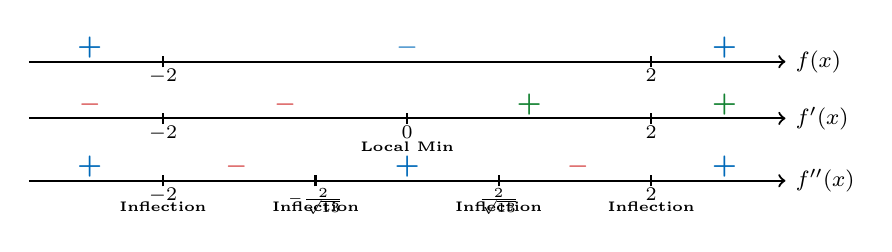
\begin{tikzpicture}[xscale=1.55, yscale=0.72]
  % f(x) number line
  \draw[thick, ->] (-3.1, 2.0) -- (3.1, 2.0) node[right] {\footnotesize $f(x)$};
  \draw[thick] (-2, 1.9) -- (-2, 2.1) node[below=1pt] {\scriptsize $-2$};
  \draw[thick] (2, 1.9) -- (2, 2.1) node[below=1pt] {\scriptsize $2$};
  \node at (-2.6, 2.25) {\textcolor{chalkblue}{\textbf{+}}};
  \node at (0, 2.25) {\textcolor{chalkblue}{\textbf{$-$}}};
  \node at (2.6, 2.25) {\textcolor{chalkblue}{\textbf{+}}};

  % f'(x) number line
  \draw[thick, ->] (-3.1, 1.0) -- (3.1, 1.0) node[right] {\footnotesize $f'(x)$};
  \draw[thick] (-2, 0.9) -- (-2, 1.1) node[below=1pt] {\scriptsize $-2$};
  \draw[thick] (0, 0.9) -- (0, 1.1) node[below=1pt] {\scriptsize $0$};
  \draw[thick] (2, 0.9) -- (2, 1.1) node[below=1pt] {\scriptsize $2$};
  \node at (-2.6, 1.25) {\textcolor{chalkred}{\textbf{$-$}}};
  \node at (-1.0, 1.25) {\textcolor{chalkred}{\textbf{$-$}}};
  \node at (1.0, 1.25) {\textcolor{chalkgreen}{\textbf{+}}};
  \node at (2.6, 1.25) {\textcolor{chalkgreen}{\textbf{+}}};
  \node at (0, 0.5) {\tiny \textbf{Local Min}};

  % f''(x) number line
  \draw[thick, ->] (-3.1, -0.1) -- (3.1, -0.1) node[right] {\footnotesize $f''(x)$};
  \draw[thick] (-2, -0.2) -- (-2, 0.0) node[below=1pt] {\scriptsize $-2$};
  \draw[thick] (-0.75, -0.2) -- (-0.75, 0.0) node[below=1pt] {\tiny $-\frac{2}{\sqrt{13}}$};
  \draw[thick] (0.75, -0.2) -- (0.75, 0.0) node[below=1pt] {\tiny $\frac{2}{\sqrt{13}}$};
  \draw[thick] (2, -0.2) -- (2, 0.0) node[below=1pt] {\scriptsize $2$};
  \node at (-2.6, 0.15) {\textcolor{chalkblue}{\textbf{+}}};
  \node at (-1.4, 0.15) {\textcolor{chalkred}{\textbf{$-$}}};
  \node at (0, 0.15) {\textcolor{chalkblue}{\textbf{+}}};
  \node at (1.4, 0.15) {\textcolor{chalkred}{\textbf{$-$}}};
  \node at (2.6, 0.15) {\textcolor{chalkblue}{\textbf{+}}};
  \node at (-2, -0.55) {\tiny \textbf{Inflection}};
  \node at (-0.75, -0.55) {\tiny \textbf{Inflection}};
  \node at (0.75, -0.55) {\tiny \textbf{Inflection}};
  \node at (2, -0.55) {\tiny \textbf{Inflection}};
\end{tikzpicture}
\end{center}

\vspace{-4pt}
\textbf{Conclusion}: All four candidate roots ($x = -2, -\frac{2}{\sqrt{13}}, \frac{2}{\sqrt{13}}, 2$) exhibit sign changes in $f''(x)$. Therefore, \textbf{all four points are true inflection points}!

\end{document}
